\documentclass[conference]{IEEEtran}
\IEEEoverridecommandlockouts
% The preceding line is only needed to identify funding in the first footnote. If that is unneeded, please comment it out.
\usepackage{cite}
\usepackage{amsmath,amssymb,amsfonts}
\usepackage{algorithmic}
\usepackage{graphicx}
\usepackage{textcomp}
\usepackage{xcolor}
\usepackage[utf8]{inputenc}
\usepackage[T1]{fontenc}
\usepackage[vietnamese]{babel}

\def\BibTeX{{\rm B\kern-.05em{\sc i\kern-.025em b}\kern-.08em
    T\kern-.1667em\lower.7ex\hbox{E}\kern-.125emX}}
\begin{document}

\title{Tạo sinh chú thích ảnh với cơ chế chú ý\\
{\footnotesize Trường Đại Học Khoa Học Tự Nhiên, thành phố Hồ Chí Minh, Việt Nam\\}
}

\author{\IEEEauthorblockN{21120127 Lê Hoàng Sơn}
\IEEEauthorblockA{\textit{VNUHCM} \\
\textit{HCMUS}\\
tp Hồ Chí Minh, Việt Nam \\
21120127@student.hcmus.edu.vn}
\and
\IEEEauthorblockN{21120085 Võ Gia Khang}
\IEEEauthorblockA{\textit{VNUHCM} \\
\textit{HCMUS}\\
tp Hồ Chí Minh, Việt Nam \\
21120085@student.hcmus.edu.vn}
}

\maketitle

\begin{abstract}
Tài liệu này mô tả xây dựng và huấn luyện mô hình phát sinh chú thích ảnh có chú ý. Mô hình này được xậy dựng dựa trên kiến trúc Encoder, Decoder và Attention Mechanism trên tập dữ liệu Flickr8k. Bên cạch đó, chúng ta sẽ thử nghiệm cải tiến mô hình.
\end{abstract}

\begin{IEEEkeywords}
Show, Tell, and Attend: Image Captioning with Attention Mechanism
\end{IEEEkeywords}

\section{Giới thiệu}
Chú thích hình ảnh nhằm mục đích tự động tạo ra các câu mô tả cho hình ảnh, chụp các đối tượng và mối quan hệ của chúng. Nhiệm vụ đầy thách thức này kết nối Thị giác máy tính (CV) và Xử lý ngôn ngữ tự nhiên (NLP) trong Trí tuệ nhân tạo (AI).
Những tiến bộ gần đây, chẳng hạn như các mô hình dựa trên sự chú ý, đã tạo ra những kết quả mạnh mẽ, cho phép các ứng dụng như công cụ trợ năng và gắn thẻ nội dung. Trong dự án này, chúng tôi triển khai một mô hình chú thích hình ảnh bằng cách sử dụng khuôn khổ CNN-RNN với sự chú ý trực quan, lấy cảm hứng từ 'Show, Attend and Tell' và tinh chỉnh nó trên tập dữ liệu Flickr8k để cải thiện chất lượng chú thích trong hơn 6 tuần.\\
Bài toán có thể được mô tả như sau: Cho ảnh đầu vào với 03 kênh màu RGB, mô hình sẽ tạo ra một câu mô tả cho ảnh đó bằng ngôn ngữ Tiếng Anh và ở hiện tại đơn. Ví dụ, ảnh đầu vào "chú chó với nền cỏ xanh" thì mô hình sẽ có thể tạo sinh ra chú thích mô tả ngắn gọn "A dog sits on green grass".\\

\section{Công trình liên quan}

\subsection{Show, Attend and Tell}
Show, Attend and Tell \cite{show_attend_tell} giới thiệu cơ chế chú ý cho phép mô hình tập trung vào các vùng quan trọng của hình ảnh. Mô hình sử dụng kiến trúc CNN (encoder) và LSTM (decoder) với cơ chế chú ý trực quan, cho phép nó tự học cách tập trung vào các phần liên quan của hình ảnh khi tạo ra từng từ trong chú thích.

\subsection{A PyTorch Tutorial to Image Captioning}
Một triển khai thân thiện với người mới bắt đầu cho mô hình chú thích hình ảnh bằng PyTorch \cite{pytorch_tutorial} cung cấp cách thực hiện CNN + LSTM với cơ chế chú ý. Dự án này sử dụng tập dữ liệu Flickr8k/COCO và cung cấp mã nguồn mở, hướng dẫn chi tiết giúp hiểu rõ quy trình xây dựng mô hình chú thích hình ảnh.

\subsection{Show and Tell}
Show and Tell \cite{show_tell} là mô hình sớm hơn sử dụng kiến trúc CNN + LSTM không có cơ chế chú ý. Đây được coi là mô hình cơ sở để so sánh hiệu quả của các mô hình sau này có tích hợp cơ chế chú ý. Mô hình này đã đặt nền tảng cho các phương pháp tiên tiến hơn trong lĩnh vực chú thích hình ảnh tự động.

% Cần thêm các tham chiếu sau vào phần tài liệu tham khảo
% \bibitem{show_attend_tell} K. Xu et al., "Show, Attend and Tell: Neural Image Caption Generation with Visual Attention," arXiv:1502.03044, 2015.
% \bibitem{pytorch_tutorial} S. G. Vinod, "A PyTorch Tutorial to Image Captioning," GitHub repository, 2018.
% \bibitem{show_tell} O. Vinyals et al., "Show and Tell: A Neural Image Caption Generator," arXiv:1411.4555, 2014.

\section{Phương pháp}
\subsection{Mô hình}
\begin{figure}[htbp]
    \centering
    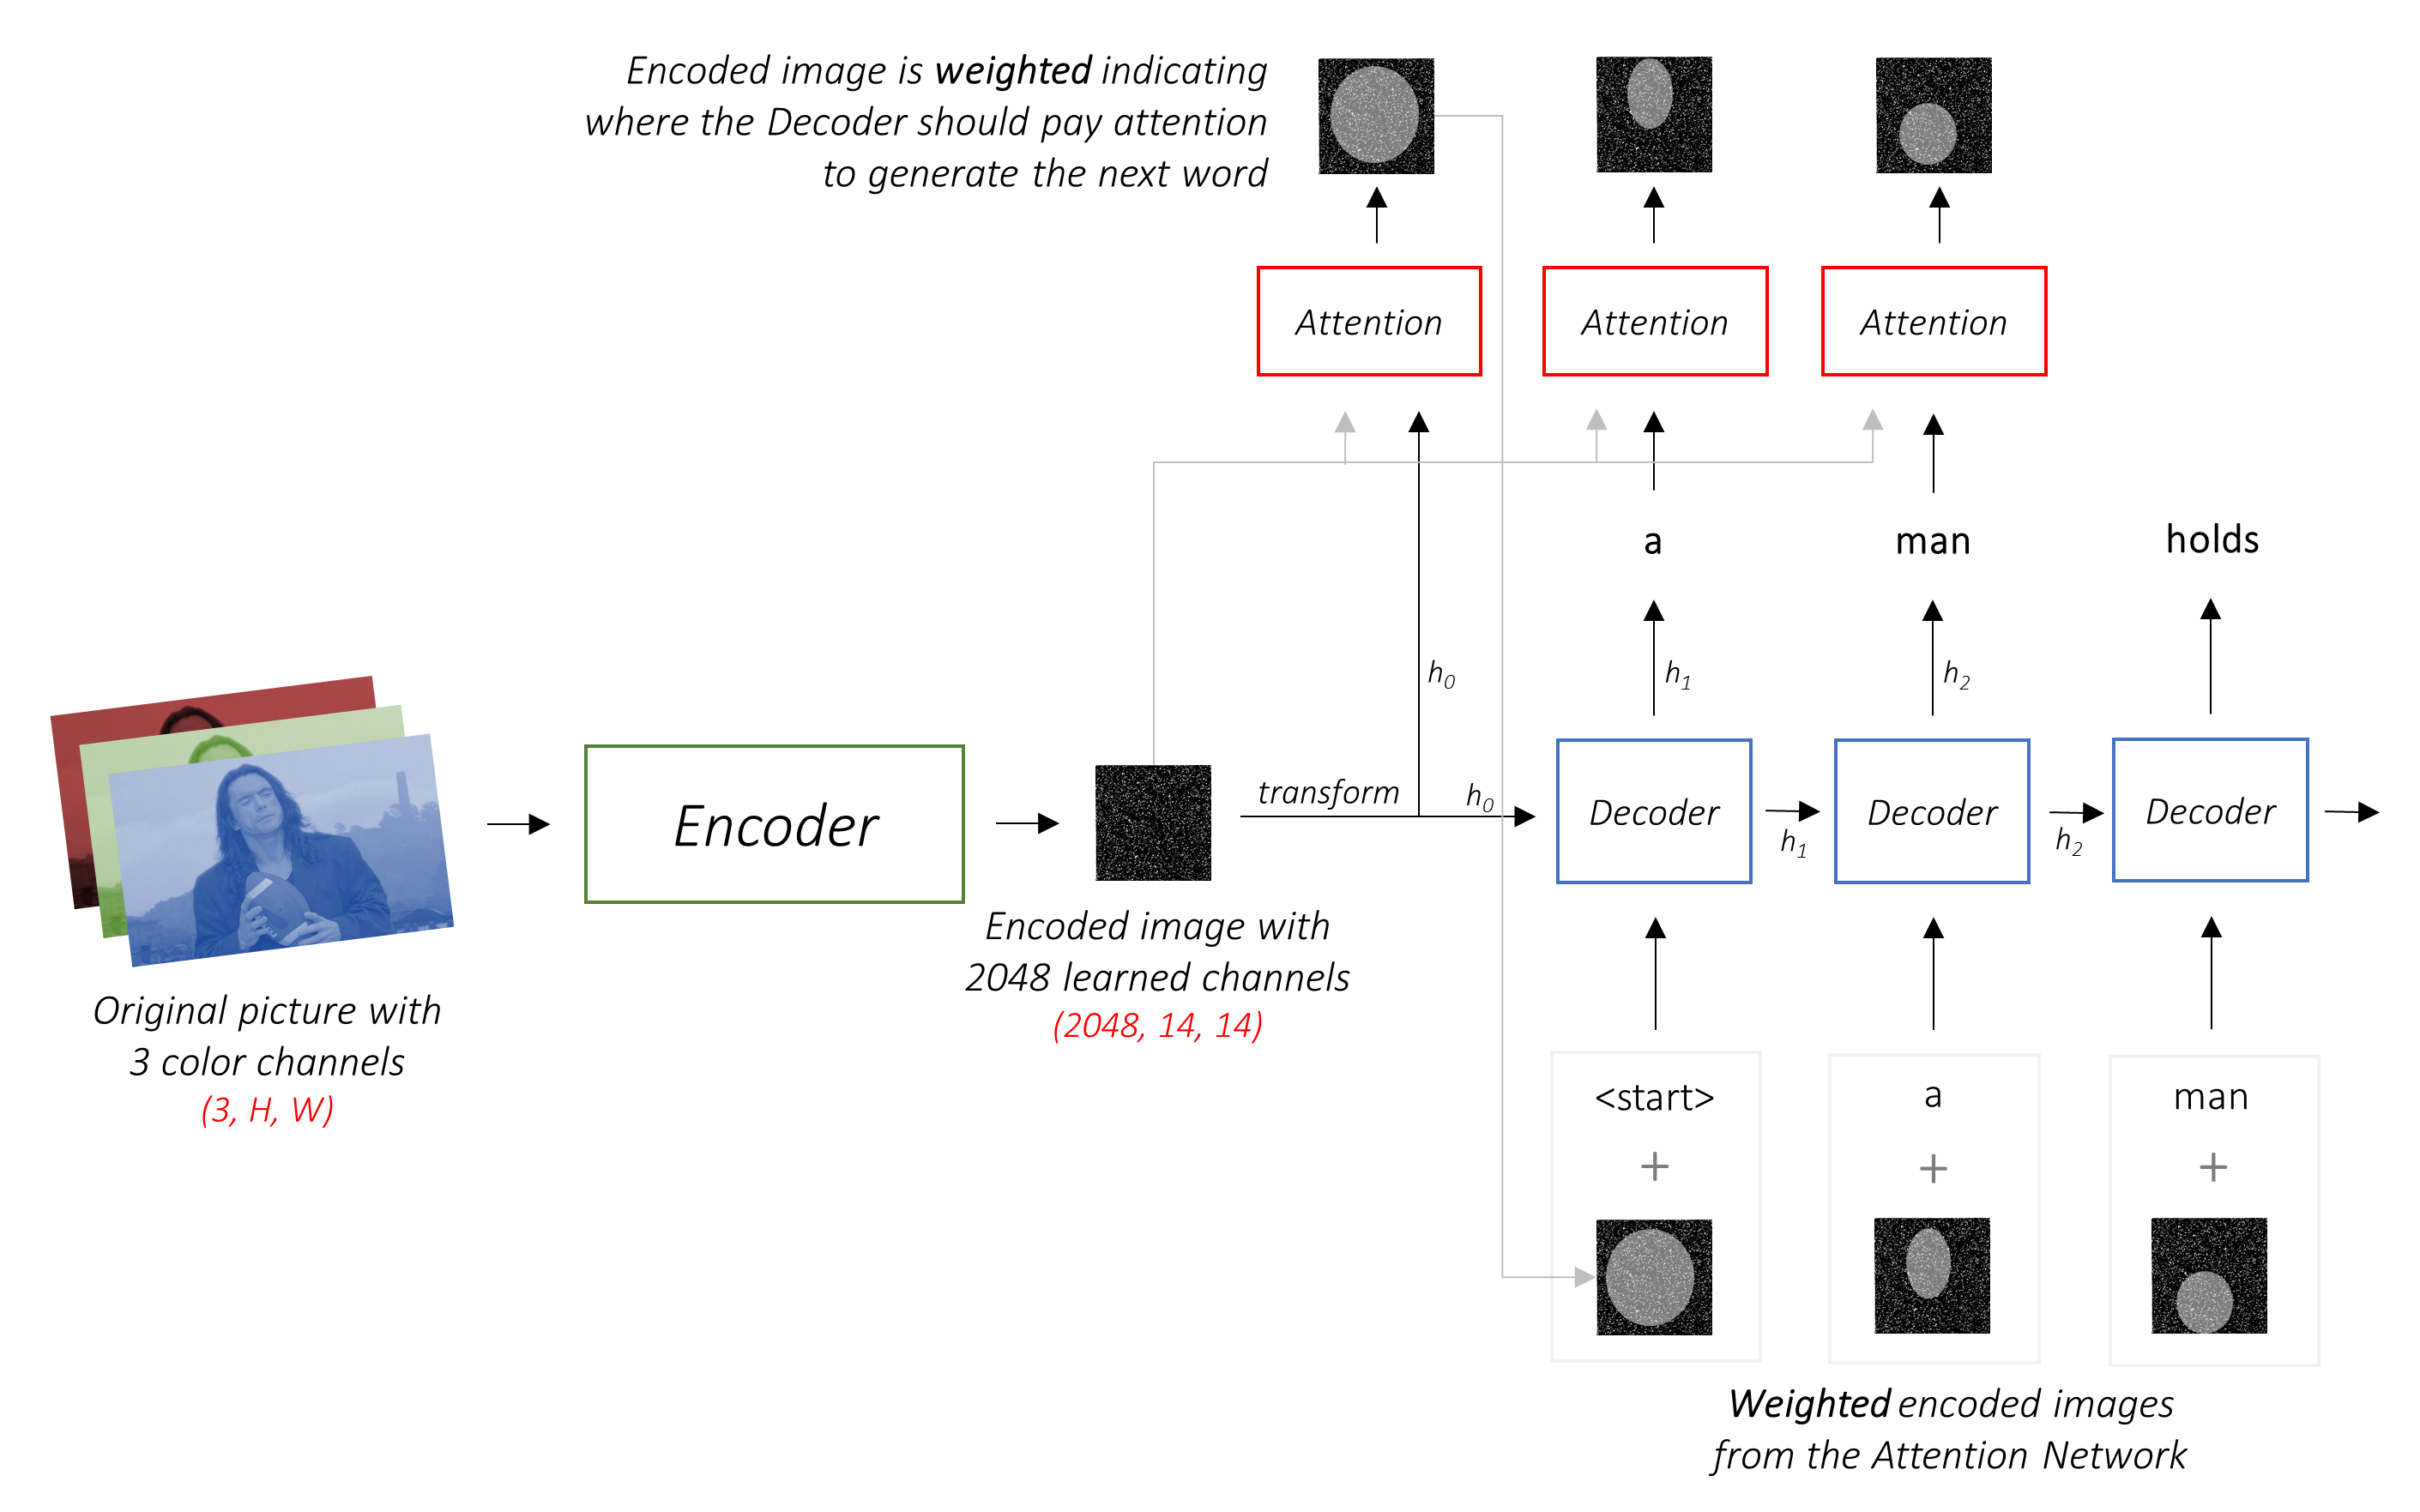
\includegraphics[width=\linewidth]{attachments/model.png}
    \caption{Kiến trúc tổng thể của mô hình Image Captioning với cơ chế chú ý, bao gồm Encoder CNN (ResNet-101), cơ chế Attention và Decoder LSTM.}
    \label{fig:model}
\end{figure}
\subsubsection{Encoder}
Chúng tôi sử dụng mô hình ResNet-101 đã được tiền huấn luyện làm bộ mã hóa để trích xuất đặc trưng từ ảnh đầu vào. Cụ thể:
\begin{itemize}
    \item Loại bỏ hai lớp cuối cùng của ResNet-101 (lớp fully-connected và lớp pooling) vì chúng tôi chỉ cần các đặc trưng chứ không cần phân loại ảnh
    \item Sử dụng Adaptive Average Pooling để chuẩn hóa kích thước đầu ra thành $14 \times 14$
    \item Đầu ra có kích thước $(batch\_size, 2048, 14, 14)$ sau đó được chuyển thành $(batch\_size, 14, 14, 2048)$ để phù hợp với bộ giải mã
    \item Cho phép tinh chỉnh (fine-tune) các khối tích chập từ 5 trở đi khi cần thiết
\end{itemize}

\subsubsection{Attention}
Cài đặt cơ chế chú ý bằng các lớp tuyến tính đơn giản để mô hình học cách tập trung vào các phần quan trọng của ảnh khi tạo từng từ.\\
Theo như tác giả Show, Attend and Tell, chúng tôi sẽ sử dụng cơ chế chú ý mềm (soft attention) để tính toán trọng số cho các phần khác nhau của ảnh. Cơ chế chú ý này sẽ giúp mô hình xác định vùng nào của ảnh là quan trọng nhất cho từng từ trong câu mô tả.\\
Cơ chế chú ý sẽ được thực hiện bằng cách sử dụng một lớp tuyến tính để tính toán trọng số cho các đặc trưng của ảnh, sau đó kết hợp chúng với đầu vào của bộ giải mã. Trọng số này sẽ được cập nhật trong quá trình huấn luyện để tối ưu hóa mô hình.
Cơ chế chú ý được triển khai gồm các thành phần:
\begin{itemize}
    \item Ba lớp tuyến tính để biến đổi:
    \begin{itemize}
        \item Đặc trưng ảnh $(encoder\_att)$
        \item Trạng thái ẩn của bộ giải mã $(decoder\_att)$
        \item Kết hợp thông tin để tính trọng số chú ý $(full\_att)$
    \end{itemize}
    \item Hàm kích hoạt ReLU và Softmax để tính trọng số chú ý
    \item Đầu vào: Đặc trưng ảnh $(encoder\_out)$ và trạng thái ẩn hiện tại của bộ giải mã $(decoder\_hidden)$
    \item Đầu ra: Mã hóa có trọng số chú ý $(attention\_weighted\_encoding)$ và ma trận trọng số chú ý $(\alpha)$
\end{itemize}

\subsubsection{Decoder}
Bộ giải mã sử dụng LSTM với cơ chế chú ý gồm các thành phần chính:
\begin{itemize}
    \item Khởi tạo trạng thái ẩn $(h, c)$ từ đặc trưng ảnh trung bình
    \item Lớp embedding để chuyển từ ngữ cảnh thành vector
    \item Tế bào LSTM $(LSTMCell)$ xử lý kết hợp:
    \begin{itemize}
        \item Embedding của từ hiện tại
        \item Mã hóa có trọng số chú ý
    \end{itemize}
    \item Cổng điều chỉnh $(f\_beta$ với $sigmoid)$ để kiểm soát ảnh hưởng của cơ chế chú ý
    \item Lớp fully-connected cuối cùng để dự đoán từ tiếp theo
    \item Quy trình hoạt động:
    \begin{itemize}
        \item Sắp xếp dữ liệu theo độ dài chú thích giảm dần
        \item Với mỗi bước thời gian:
        \begin{itemize}
            \item Tính trọng số chú ý và mã hóa có trọng số
            \item Cập nhật trạng thái LSTM
            \item Dự đoán từ tiếp theo
        \end{itemize}
        \item Chỉ xử lý các mẫu còn hoạt động (chưa kết thúc)
    \end{itemize}
\end{itemize}

Các kỹ thuật hỗ trợ:
\begin{itemize}
    \item Dropout để tránh overfitting
    \item Khởi tạo trọng số đồng đều trong khoảng $[-0.1, 0.1]$
    \item Xử lý độ dài thay đổi của chú thích
\end{itemize}
\subsection{Hàm mất mát}
Hàm mất mát được sử dụng trong mô hình này là hàm mất mát chéo entropy, giúp đo lường sự khác biệt giữa phân phối xác suất dự đoán và phân phối xác suất thực tế. Hàm mất mát này sẽ được tối ưu hóa trong quá trình huấn luyện để cải thiện độ chính xác của mô hình.

\subsection{Đánh giá}

Đánh giá mô hình sẽ được thực hiện bằng cách sử dụng chỉ số BLEU, một phương pháp phổ biến để đo lường chất lượng của các mô tả được tạo ra so với các mô tả tham chiếu. Chỉ số BLEU sẽ giúp chúng tôi đánh giá độ chính xác và tính tự nhiên của các câu mô tả.
Ngoài ra, chúng tôi cũng sẽ sử dụng chỉ số METEOR để đánh giá chất lượng mô tả. Chỉ số này tính toán sự tương đồng giữa các từ trong câu được tạo ra và các từ trong câu tham chiếu, bao gồm cả các yếu tố ngữ nghĩa và ngữ pháp.

\section{Kế hoạch}
\subsection{Tổng quan}
Dự án này được thực hiện trong khoảng thời gian 6 tuần, trong đó chúng tôi lập kế hoạch triển khai và cải tiến mô hình chú thích hình ảnh dựa trên kiến trúc Encoder-Attention-Decoder.
\subsection{Kiến trúc đề xuất}
Mô hình của chúng tôi sẽ sử dụng kiến trúc tương tự như "Show, Attend and Tell":
\begin{itemize}
    \item \textbf{Encoder}: Sử dụng Convolutional Neural Network (ResNet-101) để trích xuất đặc trưng từ ảnh, tạo ra L vector đại diện cho các phần khác nhau của ảnh, mỗi vector có chiều D.
    \item \textbf{Attention}: Cài đặt cơ chế chú ý bằng các lớp tuyến tính đơn giản để mô hình học cách tập trung vào các phần quan trọng của ảnh khi tạo từng từ.
    \item \textbf{Decoder}: Sử dụng Long Short-Term Memory (LSTM) để tạo ra câu mô tả từ các đặc trưng đã được trích xuất và thông tin chú ý.
\end{itemize}

\subsection{Tiến độ thực hiện}
\begin{itemize}
    \item \textbf{Tuần 1-2}: Thu thập và tiền xử lý dữ liệu Flickr8k, xây dựng pipeline dữ liệu
    \item \textbf{Tuần 3-4}: Cài đặt mô hình cơ bản (Encoder-Decoder) không có cơ chế chú ý
    \item \textbf{Tuần 4-5}: Tích hợp cơ chế chú ý và tối ưu hóa mô hình
    \item \textbf{Tuần 5-6}: Đánh giá mô hình sử dụng BLEU score và thực hiện cải tiến
\end{itemize}

\subsection{Cải tiến dự kiến}
\begin{itemize}
    \item Thử nghiệm với các mạng CNN khác nhau cho Encoder (ResNet, Inception-v3)
\end{itemize}

\section{Huấn luyện và phân tích mô hình}
\subsection{Mô tả bộ dữ liệu}

Dữ liệu được sử dụng trong mô hình này là tập dữ liệu Flickr8k, bao gồm 8,000 hình ảnh và các mô tả tương ứng. Tập dữ liệu này được chia thành các phần huấn luyện, kiểm tra và xác thực để đảm bảo mô hình có thể học và đánh giá hiệu quả.\\
Tuy nhiên, ở đây chúng tôi sẽ sử dụng bộ mô tả ảnh của Andrej Karpathy \cite{pytorch_tutorial} với 8,000 hình ảnh và 40,000 mô tả. Mỗi hình ảnh có 5 mô tả khác nhau, giúp mô hình học được nhiều cách diễn đạt khác nhau cho cùng một nội dung.\\
Để chuẩn bị dữ liệu cho mô hình, chúng tôi đã thực hiện các bước sau:
\begin{itemize}
    \item Xây dựng Worldmap, ánh xạ các từ trong mô tả thành các chỉ số số nguyên.
    \item Tổ chức dữ liệu thành tập huân luyện và kiểm tra dưới định dạng hdf5 để dễ dàng truy cập và xử lý.
    \item Thêm từ đặc biệt như <start> và <end> để đánh dấu bắt đầu và kết thúc của một mô tả.
\end{itemize}

\subsection{Kết quả đánh giá}

Chúng tôi đã đánh giá mô hình trên tập dữ liệu Flickr8k sử dụng các chỉ số BLEU và METEOR. Kết quả đạt được với beam size là 1 như sau:

\begin{table}[h]
\centering
\begin{tabular}{|c|c|}
\hline
\textbf{Chỉ số} & \textbf{Giá trị} \\
\hline
BLEU-1 & 0.6282 \\
\hline
BLEU-2 & 0.4484 \\
\hline
BLEU-3 & 0.3108 \\
\hline
BLEU-4 & 0.2084 \\
\hline
METEOR & 0.4197 \\
\hline
\end{tabular}
\caption{Kết quả đánh giá mô hình trên tập dữ liệu Flickr8k với beam size là 1}
\label{tab:evaluation}
\end{table}

Các chỉ số BLEU đánh giá độ chính xác của n-grams (1, 2, 3, và 4 từ liên tiếp) trong câu được tạo ra so với câu tham chiếu. Chỉ số METEOR đánh giá dựa trên sự tương đồng của từng từ, đồng nghĩa, và các yếu tố ngôn ngữ học khác. Kết quả cho thấy mô hình của chúng tôi hoạt động tương đối tốt, đặc biệt với BLEU-1 và METEOR.

\section{Cải tiến mô hình}
\subsection{Các cải tiến đang thực hiện}

Hiện tại, chúng tôi đang tiếp tục cải tiến mô hình để nâng cao hiệu suất và khả năng tạo sinh chú thích.

\section{Thực nghiệm}
Ở phần này, chúng tôi sẽ chạy thử nghiệm một vài mẫu ảnh để kiểm tra mô hình đã được huấn luyện. Chúng tôi sẽ sử dụng một số ảnh từ tập dữ liệu Flickr8k và một số ảnh ngẫu nhiên khác để kiểm tra khả năng tạo sinh chú thích của mô hình.
\subsection{Thử nghiệm với các ảnh mẫu}

\begin{center}
    \begin{minipage}[b]{0.48\textwidth}
        \centering
        \includegraphics[width=\linewidth]{attachments/test00.jpg}
        \vspace{0.2cm}
        \textbf{Ảnh mẫu thử nghiệm 1}
    \end{minipage}
    \hfill
    \begin{minipage}[b]{0.48\textwidth}
        \centering
        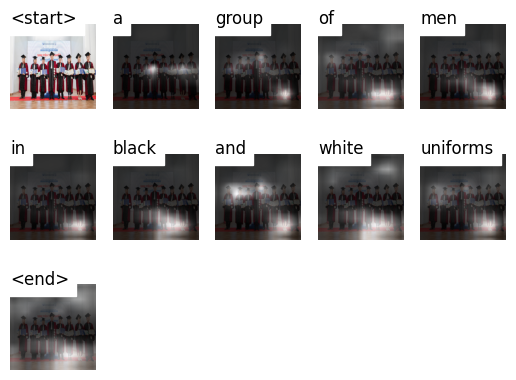
\includegraphics[width=\linewidth]{attachments/test00_caption.jpg}
        \vspace{0.2cm}
        \textbf{Chú thích được tạo ra cho ảnh mẫu 1}
    \end{minipage}
\end{center}

\vspace{1cm}

\begin{center}
    \begin{minipage}[b]{0.48\textwidth}
        \centering
        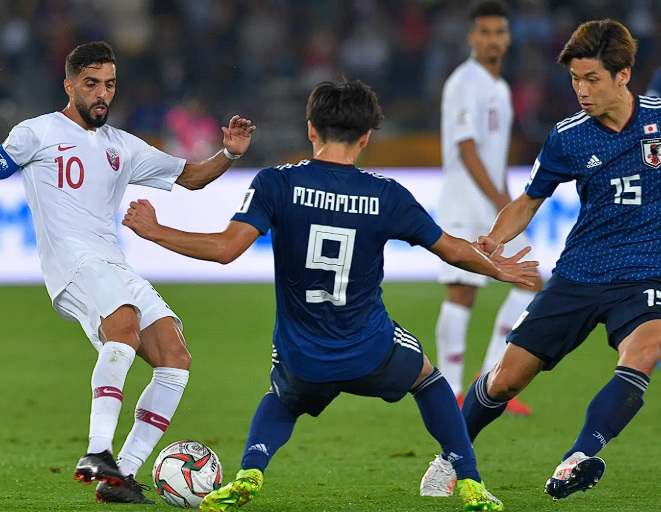
\includegraphics[width=\linewidth]{attachments/test01.jpg}
        \vspace{0.2cm}
        \textbf{Ảnh mẫu thử nghiệm 2}
    \end{minipage}
    \hfill
    \begin{minipage}[b]{0.48\textwidth}
        \centering
        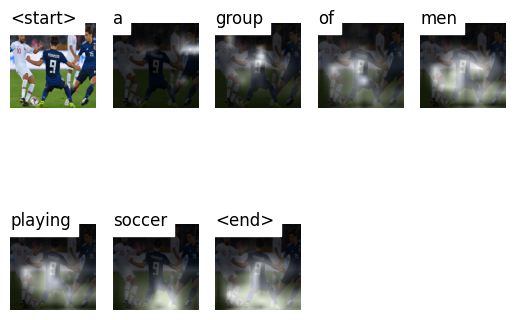
\includegraphics[width=\linewidth]{attachments/test01_caption.jpg}
        \vspace{0.2cm}
        \textbf{Chú thích được tạo ra cho ảnh mẫu 2}
    \end{minipage}
\end{center}

\subsection{Phân tích kết quả}
Từ các kết quả thử nghiệm trên, chúng ta có thể thấy mô hình đã học được cách tạo ra chú thích phù hợp cho các ảnh đầu vào. Mô hình có khả năng nhận diện các đối tượng chính trong ảnh và mô tả hành động của chúng một cách chính xác. Tuy nhiên, vẫn có một số trường hợp mô hình chưa mô tả đầy đủ hoặc chính xác hoàn toàn chi tiết trong ảnh, cho thấy còn dư địa để cải thiện trong tương lai.
\section{Kết luận}

\begin{thebibliography}{00}
\bibitem{show_attend_tell} K. Xu et al., "Show, Attend and Tell: Neural Image Caption Generation with Visual Attention," arXiv:1502.03044, 2015.
\bibitem{pytorch_tutorial} S. G. Vinod, "A PyTorch Tutorial to Image Captioning," GitHub repository, 2018.
\bibitem{show_tell} O. Vinyals et al., "Show and Tell: A Neural Image Caption Generator," arXiv:1411.4555, 2014.
\end{thebibliography}
\vspace{12pt}
\color{red}

\end{document}